\footnotetext{Notes from Classical Mechanics by John R. Taylor, ch. 6}

\section{Two example problems}
The calculus of variations can be used to find a function $y(x)$ that minimizes a scalar quantity
that is expressed as an integral $\int_{x_0}^{x_1} f[y(x), y'(x), x] \dx$. Here are two such
problems:

\begin{question*}
  What is the shortest path between two points in a plane?
\end{question*}

\begin{proof}
  Let the points be $(x_0, y_0)$ and $(x_1, y_1)$ and let them be joined by some path $y(x)$ of
  length $S$. Consider a short section of the path of length $\Delta s$ above a section of the
  $x$-axis of length $\Delta x$, and make a linear approximation to the path in this region. The
  length of the hypotenuse is
  \begin{align*}
    \Delta s = \sqrt{(\Delta x)^2 + (y'(x)\Delta x)^2} = \sqrt{1 + y'(x)^2} \Delta x.
  \end{align*}
  Therefore a shortest path is a function $y(x)$ that minimizes
  \begin{align*}
    S = \int_{x_0}^{x_1} \d s = \int_{x_0}^{x_1} \sqrt{1 + y'(x)^2} \dx,
  \end{align*}
  with the constraint that the endpoints are fixed at $y(x_0) = y_0$ and $y(x_1) = y_1$.

  \todo{Find the function $y$ that minimizes this integral.}
\end{proof}


\begin{question*}
  In 1662 Fermat proposed that light, when passing from one point to another through a material with
  varying refractive index, takes the path which takes least time\footnote{\todo{In fact, the path
      taken is a stationary point with respect to the action? time? ...not necessarily least}}. What
  is this path?
\end{question*}

\begin{proof}
  Again consider a short section of the path of length $\Delta s$ above a section of the $x$-axis of
  length $\Delta x$. Let $c$ be the speed of light and $n$ be the refractive index in this
  region. This means that the light travels at speed $c/n$, and therefore takes time $(n/c)\Delta s$
  to pass along the hypotenuse. The refractive index $n$ can vary with both $x$ and $y$, therefore a
  least-time path is a function $y(x)$ that minimizes
  \begin{align*}
    T = \int_{x_0}^{x_1} n(x, y(x)) \d s = \int_{x_0}^{x_1} n(x, y(x)) \sqrt{1 + y'(x)^2} \dx,
  \end{align*}
  with the constraint that the endpoints are fixed at $y(x_0) = y_0$ and $y(x_1) = y_1$.

  \todo{Find the function $y$ that minimizes this integral.}
\end{proof}

A naive thought would be to somehow treat $y$ similarly to how a variable is treated when minimizing
a function in in basic calculus, i.e. differentiate the expression with respect to $y$. Recall that
the definition of derivative is
\begin{align*}
  f'(y_0) = \lim_{y_1 \to y_0}\frac{f(y_1) - f(y_0)}{||y_1 - y_0||}.
\end{align*}

\todo{I think this is nonsense and the reason is that multiplication (and therefore division) of
  functions is not defined (they can be treated as vectors, so can be added and scaled, but do not
  have an obviously appropriate multiplication operation). I don't think choosing a norm would
  necessarily be problematic.}

\section{The Euler-Lagrange equations}

\begin{proof}
  Note that in both example problems, the integral to be minimized can be viewed as a scalar-valued
  \emph{functional} $f$ that depends on the \emph{functions} $y(x)$ and $y'(x)$\footnote{It seems to
    me that this could also be written as $S[y, y'] = \int _{x_0}^{x_1} f[y(x), y'(x)](x) \dx$}:
  \begin{align*}
    S(y, y') = \int_{x_0}^{x_1} f[y(x), y'(x), x] \dx.
  \end{align*}

  We'll refer to $S$ as giving the \emph{cost} of traveling along the path $y$, from $(x_0, y_0)$ to
  $(x_1, y_1)$. Of course, $y$ and $y'$ are not independent variables, so we could just write $S(y)$.
  However, we won't: we'll write $S(y, y')$.

  Recall that we seek a least-cost path $y(x)$, subject to the requirement that the endpoints are
  $y(x_0) = y_0$ and $y(x_1) = y_1$. Let $y(x)$ be the least-cost path, and consider an alternative
  path $Y(x)$ whose cost is greater than that of $y(x)$. We can write $Y(x)$ as
  \begin{align*}
    Y(x) = y(x) + \eta(x),
  \end{align*}
  where the difference function $\eta$ must satisfy $\eta(x_0) = \eta(x_1) = 0$.  Now introduce a
  parameter $\alpha$ and redefine $Y(x)$ as
  \begin{align*}
    Y(x) = y(x) + \alpha\eta(x).
  \end{align*}
  So now we have a family of paths, parameterized by $\alpha$, all satisfying the endpoint requirement,
  and with the least-cost path corresponding to $\alpha=0$. We can consider the cost of these paths to
  be a function $S(\alpha)$:
  \begin{align*}
    S(\alpha) &= \int_{x_0}^{x_1} f(Y, Y', x) \dx \\
              &= \int_{x_0}^{x_1} f\(y(x) + \alpha\eta(x), y'(x) + \alpha\eta'(x), x\) \dx.
  \end{align*}
  We are trying to find a $y(x)$ that is a minimum in the cost surface over the function space (or a
  maximum, or saddle point). For such a $y(x)$ it must be the case that
  \begin{align*}
    \pdv{S}{\alpha}\Big|_{\alpha=0} = 0.
  \end{align*}
  So, let's compute $\pdv*{S}{\alpha}$ and use the fact that it must evaluate to zero at $\alpha=0$
  to obtain an equation that $y$ must obey. We'll assume that $f$ satisfies the (mild) conditions
  necessary to differentiate under the integral sign, i.e. that
  \begin{align*}
    \pdv{S}{\alpha} = \pdv{}{\alpha}\int_{x_0}^{x_1} f(Y, Y', x) \dx
                    = \int_{x_0}^{x_1} \pdv{f(Y, Y', x)}{\alpha} \dx.
  \end{align*}
  Dropping the explicit function notation, we have
  \begin{align*}
    Y  &= y + \alpha\eta \\
    Y' &= y' + \alpha\eta',
  \end{align*}
  and so from the chain rule we have\footnote{It seems to me that this is the first time (?) that we
    are treating functions ($\eta$ and $\eta'$) as objects on which a multiplication operation is
    defined. I.e. we're saying that $\dv{}{\alpha}\alpha\eta = \eta$, as if $\eta$ were a simple
    scalar from a field.}
  \begin{align*}
    \pdv{f(Y, Y', x)}{\alpha} &= \pdv{f}{Y}\pdv{Y}{\alpha} + \pdv{f}{Y'}\pdv{Y'}{\alpha} \\
                              &= \pdv{f}{Y}\eta + \pdv{f}{Y'}\eta'.
  \end{align*}
  Plugging this into the expression for $\pdv*{S}{\alpha}$ and evaluating at $\alpha = 0$ we have
  \begin{align*}
    \int_{x_0}^{x_1} \(\eta\pdv{f}{y} + \eta'\pdv{f}{y'}\) \d x = 0.
  \end{align*}
  (I believe that $Y$ and $Y'$ have now become $y$ and $y'$ because we are evaluating at
  $\alpha=0$.)

  Now, recall integration by parts,
  $\int_a^b u \dv{v}{x} \d x = [uv]_a^b - \int_a^b v\dv{u}{x}\d x$, and apply it to the second term
  inside the integral:
  \begin{align*}
    \int_{x_0}^{x_1} \eta'\pdv{f}{y'} \d x = \Bigg[\eta\pdv{f}{y'}\Bigg]_{x_0}^{x_1} - \int_{x_0}^{x_1} \eta\(\dv{}{x}\pdv{f}{y'}\)\d x.
  \end{align*}
  Because $\eta$ was defined to be the difference between two candidate paths, as noted above we
  have that $\eta(x_0) = \eta(x_1) = 0$. Thus the first term (the ``endpoint term'' or ``boundary
  term'') is zero\footnote{According to Taylor this is common in physics, i.e. that the endpoint
    term is zero and thus integration by parts results in ``switching the prime'' from one factor to
    the other under the integral, and applying a negation.}. So now we have
  \begin{align*}
    \int_{x_0}^{x_1} \eta(x)\(\pdv{f}{y} - \dv{}{x}\pdv{f}{y'}\) \d x = 0.
  \end{align*}
  We now argue that this means that the difference-of-derivatives-function inside the integral is
  zero for all $x$. The reason is basically that this equality is true for \emph{any} $\eta(x)$. So
  suppose the difference-of-derivatives-function were not equal to zero for some $x$. Then we could
  construct an $\eta(x)$ that is non-zero for the same $x$ values that the
  difference-of-derivatives-function is non-zero for, the upshot being that we could construct
  things so that the value of the integral is non-zero; a contradiction. Therefore the
  difference-of-derivatives-function is zero for all $x$, and we have the Euler-Lagrange equations:
  \begin{align*}
    \pdv{f}{y} = \dv{}{x}\pdv{f}{y'}.
  \end{align*}
  This is a system of differential equations which must be satisfied by any path that is stationary
  with respect to $f$.
\end{proof}

\newpage
\footnote{Notes and exercises from Sussman et al. Structure and Interpretation of Classical Mechanics}
\subsubsection*{SICM ch. 1 Lagrangian Mechanics Exercise 1.4}
\begin{mdframed}
  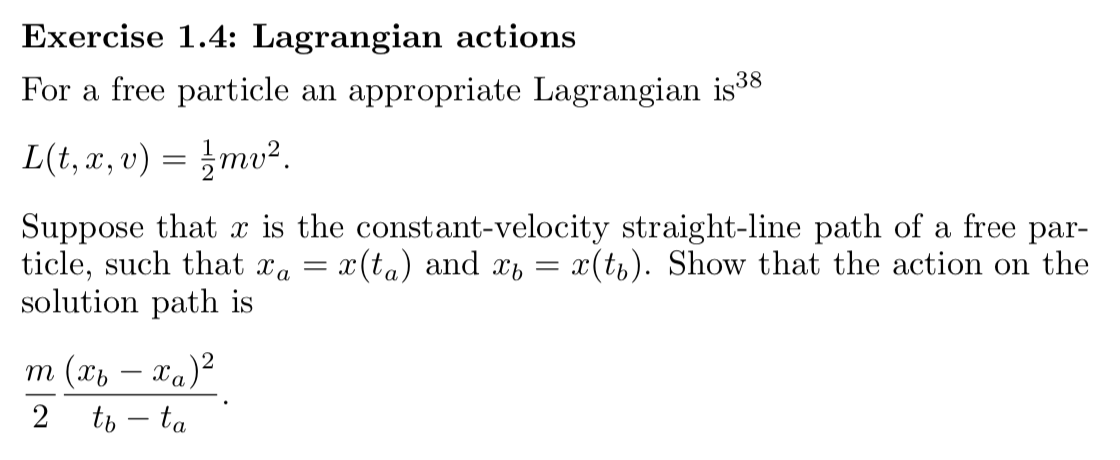
\includegraphics[width=400pt]{img/physics--classical-mechanics--sicm--1-4.png}
\end{mdframed}
The path function is
\begin{align*}
  x(t) = x_a + \frac{t - t_a}{t_b - t_a}(x_b - x_a).
\end{align*}
Therefore the velocity function is the constant function
\begin{align*}
  v(t) = (D x)(t) = \frac{x_b - x_a}{t_b - t_a}.
\end{align*}
Therefore the action is
\begin{align*}
  S[x](t_a, t_b) &= \int_{t_a}^{t_b}  \frac{1}{2}m \frac{(x_b - x_a)^2}{(t_b - t_a)^2} \d t \\
                 &= \frac{m}{2} \frac{(x_b - x_a)^2}{(t_b - t_a)^2}\int_{t_a}^{t_b} \d t \\
                 &= \frac{m}{2} \frac{(x_b - x_a)^2}{t_b - t_a}.
\end{align*}
